\documentclass[a4paper]{article}
\usepackage{tikz} % Pretty pictures, google tikzmanual.pdf
\usetikzlibrary{arrows,decorations.pathmorphing,backgrounds}
\usepackage{float}
\usepackage[english]{babel}
\usepackage[utf8x]{inputenc}
\usepackage{amsmath}
\usepackage{graphicx}
\usepackage[colorinlistoftodos]{todonotes}

\usepackage{amsthm}
\usepackage{algorithm2e}
\usepackage{algpseudocode}
\usepackage{placeins}

\newtheorem{thm}{Theorem}[section] 
\newtheorem{lem}{Lemma}[section]
\newtheorem{cor}[lem]{Corollary}

\title{Airplane Seating Problem}
\author{Algorithms Group}
\setlength{\parindent}{0mm}
\newcommand{\tab}{\hspace*{2em}}

\begin{document}
\maketitle

\begin{abstract}
While on an airplane, passengers are often asked to swap seats with another passenger so that a couple or a family can sit together.  This paper focuses on minimizing the number of passenger exchanges to make all families on a plane happy.
We give a hardness proof for the general case of unbounded, heterogeneous family sizes and optimal algorithms for smaller families on idealized planes and more realistic seating arrangements.
\end{abstract}

\section{Introduction}
Though passengers on an airplane book their seats as families, we imagine that during boarding many of these families wound up scattered throughout the plane rather than next to each other.  Since the only way to fix this situation without reboarding is single passenger exchanges (swaps), we would like to find the smallest number of swaps necessary so that all families are happily seated together.

\subsection{Airplane as a Line Simplification}

Instead of using actual airplane seating charts, we first consider the one dimensional case, where we think of the airplane seats to be arranged in a line, as shown below in figure \ref{fig:lineplane}.  All seats labeled ``A'' are initially populated with a member of the A family, ``B'' the B family, and ``C'' the C family.  You'll note from the figure that we don't care about the ordering within a family (i.e. Dad in seat 1 and Mom in seat 2 is exactly as optimal as Mom in seat 1 and Dad in seat 2). 

\begin{figure}[H]
\label{fig:lineplane}
\centering
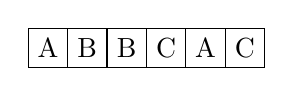
\begin{tikzpicture}[scale=1]
\draw (0,0.0) +(-.25,-.25) rectangle ++(.25,.25);
\draw (0,0.0) node{A};
\draw (0.5,0) +(-.25,-.25) rectangle ++(.25,.25);
\draw (0.5,0) node{B};
\draw (1.0,0) +(-.25,-.25) rectangle ++(.25,.25);
\draw (1.0,0) node{B};
\draw (1.5,0) +(-.25,-.25) rectangle ++(.25,.25);
\draw (1.5,0) node{C};
\draw (2.0,0) +(-.25,-.25) rectangle ++(.25,.25);
\draw (2.0,0) node{A};
\draw (2.5,0) +(-.25,-.25) rectangle ++(.25,.25);
\draw (2.5,0) node{C};
\end{tikzpicture}
\caption{Viewing an airplane as a a line of passengers.}
\end{figure}

In order to make all passengers happy in the smallest number of swaps, we first exchange seats 2 and 5 (which keeps the total number of happy families constant):

\begin{figure}[H]
\centering
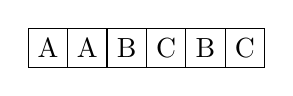
\begin{tikzpicture}[scale=1]
\draw (0,0.0) +(-.25,-.25) rectangle ++(.25,.25);
\draw (0,0.0) node{A};
\draw (0.5,0) +(-.25,-.25) rectangle ++(.25,.25);
\draw (0.5,0) node{A};
\draw (1.0,0) +(-.25,-.25) rectangle ++(.25,.25);
\draw (1.0,0) node{B};
\draw (1.5,0) +(-.25,-.25) rectangle ++(.25,.25);
\draw (1.5,0) node{C};
\draw (2.0,0) +(-.25,-.25) rectangle ++(.25,.25);
\draw (2.0,0) node{B};
\draw (2.5,0) +(-.25,-.25) rectangle ++(.25,.25);
\draw (2.5,0) node{C};
\end{tikzpicture}
\end{figure}

Then we exchange the passengers in seats 3 and 6:

\begin{figure}[H]
\centering
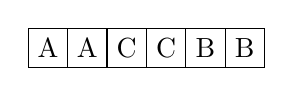
\begin{tikzpicture}[scale=1]
\draw (0,0.0) +(-.25,-.25) rectangle ++(.25,.25);
\draw (0,0.0) node{A};
\draw (0.5,0) +(-.25,-.25) rectangle ++(.25,.25);
\draw (0.5,0) node{A};
\draw (1.0,0) +(-.25,-.25) rectangle ++(.25,.25);
\draw (1.0,0) node{C};
\draw (1.5,0) +(-.25,-.25) rectangle ++(.25,.25);
\draw (1.5,0) node{C};
\draw (2.0,0) +(-.25,-.25) rectangle ++(.25,.25);
\draw (2.0,0) node{B};
\draw (2.5,0) +(-.25,-.25) rectangle ++(.25,.25);
\draw (2.5,0) node{B};
\end{tikzpicture}
\end{figure}

This second swap made 2 families happy with a single swap, and now all families are seated together. Please note that the family blocks are not in alphbetical order, and that any arrangement where all family membes are seated adjacent to each other is optimal.  

Also note that while this required only 2 swaps (the lowest possible for this input) that both swaps involved member of the ``B'' family.  Its possible to generate a pathological case where every swap involves the same passenger yet still minimizes the total number of swaps.  While this does not accurately reflect how grumpy this would make a passenger on our plane, our current model only cares about total number of swaps, future work will limit the maximum number of times a single passenger will have to swap.

\subsection{Limited Family Size Simplification}

While the general case allows passengers to fly together in arbitrarially large, heterogeneous groups, finding the optimal number of swaps in that case is NP-complete (see \ref{sec:hardness}).  Because of this, we simplify the number of people who can belong to a family in two ways: either we limit the maximum family size in a heterogeneous assortment of families, or we demand all families be the same size.  

\section{Hardness} \label{sec:hardness}

For any case of the known NP-complete problem, 3 partition, there exists an initial passenger location assignment and family size combination where finding the minimum number of swaps possible would mean solving the 3-partition problem.  The reduction follows.

The 3-partition problem is defined as: Given a set of $n = 3m$ integers $x_i$, is there a grouping of the $x_i$ into $m$ disjoint triplets so that the sum of each triplet is the same number $k$?

For any 3-partition instance, we can design the seating arrangement as follows.  There are $m$ blocking families, $B_1, B_2... B_m$ all with the very large number of family members, $M_b > mk$.  For each $x_i$ there is a single family with $x_i$ family members, call these families $f_i$.  Finally there is a single huge family, the Seatwarmers, of size $\sum_i x_i = mk$, that we label $S$.

Our initial seating arrangement is to sit exactly $k$ seatwarmers in the first seats, followed by every member of $B_1$, then alternate between placing a block of $k$ seatwarmers and family $B_i$ until we seat $B_m$ and all $mk$ seatwarmers.  After this we seat all remaining passengers in perfectly rifled order, i.e. $f_1 f_2 f_3 f_1 f_2 f_3 \hdots$.  We sketch this arrangement below (with k = 4, M=2):

\begin{figure}[H]
\centering
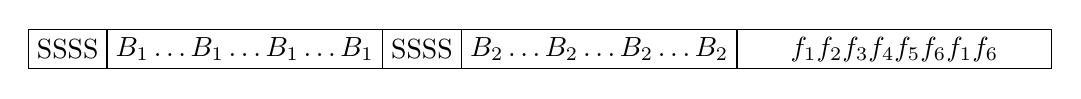
\begin{tikzpicture}[scale=1]
\draw (0,0.0) +(-.5,-.25) rectangle ++(.5,.25);
\draw (0,0.0) node{SSSS};
\draw (2.25,0) +(-1.75,-.25) rectangle ++(1.75,.25);
\draw (2.25,0) node{$B_1 \hdots B_1 \hdots B_1 \hdots B_1$};
\draw (4.5,0) +(-.5,-.25) rectangle ++(.5,.25);
\draw (4.5,0) node{SSSS};
\draw (6.75,0) +(-1.75,-.25) rectangle ++(1.75,.25);
\draw (6.75,0) node{$B_2 \hdots B_2 \hdots B_2 \hdots B_2$};
\draw (10.5,0) +(-2.0,-.25) rectangle ++(2.0,.25);
\draw (10.5,0) node{$f_1 f_2 f_3 f_4 f_5 f_6 f_1 f_6$};
\end{tikzpicture}
\end{figure}

If this problem has a 3 partition, then in exactly $mk$ swaps we can make every family happy by swapping all of the seatwarmers in to the back of the plane, leaving the blocking families in place and in between each set of blocking families putting exactly 3 full $f_i$ families.  

Our toy instance's optimal seating arrangement is:

\begin{figure}[H]
\centering
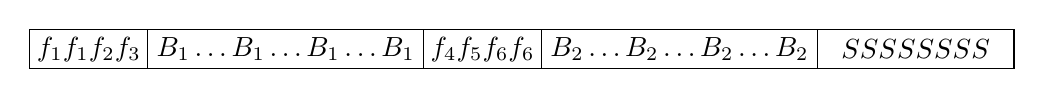
\begin{tikzpicture}[scale=1]
\draw (0,0.0) +(-.75,-.25) rectangle ++(.75,.25);
\draw (0,0.0) node{$f_1 f_1 f_2 f_3$};
\draw (2.5,0) +(-1.75,-.25) rectangle ++(1.75,.25);
\draw (2.5,0) node{$B_1 \hdots B_1 \hdots B_1 \hdots B_1$};
\draw (5.0,0) +(-.75,-.25) rectangle ++(.75,.25);
\draw (5.0,0) node{$f_4 f_5 f_6 f_6$};
\draw (7.5,0) +(-1.75,-.25) rectangle ++(1.75,.25);
\draw (7.5,0) node{$B_2 \hdots B_2 \hdots B_2 \hdots B_2$};
\draw (10.5,0) +(-1.25,-.25) rectangle ++(1.25,.25);
\draw (10.5,0) node{$SSSSSSSS$};
\end{tikzpicture}
\end{figure}

\begin{proof}[$mk$ is the minimum number of required swaps $\forall m > 2$]
If the seatwarmers all sit together in the back of the plane, it requires one swap per seatwarmer to get back there, or exactly $mk$ swaps.  

By contradiction, assume the seatwarmers don't sit in the final block in the back of the plane.  This means some members of a blocking family $B_i$ have to move.  As long as $M_B > mk$, there are more blocking members in any family than there are seatwarmers, so at most $k$ seatwarmers don't have to change their seat.  Getting the rest to sit in this unmoving block will require $(m-1)k$ swaps.

However, there are now $(m-1)k$ blocking members sitting in the wrong seats.  Since any exchange either puts 0,1 or 2 people in their optimal location, it takes a minimum of $\frac{(m-1)k}{2}$ exchanges to make these blocking members happy.  So long as $\frac{3(m-1)}{2} >= m$ or $m>=3$, this is no better than the $mk$ swaps we achieved using the initial method.
\end{proof}


\section{Solved Cases}

\subsection{Family size of exactly 2}

\noindent
Let us assume that we only have couples on-board, maybe a plane full of honeymooners headed to a post-nuptial resort. For this case, the following sweeping-line algorithm was proposed:

\begin{algorithm}
\label{alg:twoSweep}
\While{ $i \leq n-2$ }{
  Read a pair ($i$, $i+1$) 
  \If{ $couple(i) \neq couple(i+1)$}{
    let $j = i+2$
    \While{ $couple(j) \ne couple(i)$}{
      $j = j + 1$
    }
    Swap (j, i+1)
  }
}
\caption{ \texttt{Sweep algorithm for families of size two} }
\end{algorithm}
\FloatBarrier

\begin{thm} \label{thm:sweepCorrectness}
There exists an optimal set of single passenger exchanges where the leftmost position of passengers involved in each exchange is non-decreasing.
\end{thm}


If we imagine a solution to this problem as an ordered pair of seat numbers to be exchanged, $(i_1,j_1), (i_2,j_2)...$ then the following observation can be made. 

\begin{lem} \label{lem:swapRules} 
We can change the order of exchanges using the three rules (with $a,b,c,d$ being unique seat numbers) without changing the final permutation achieved by performing these swaps.

\begin{eqnarray*}
(a,b) (c,d) \rightarrow (c,d) (a,b) \\
(a,b) (a,c) \rightarrow (a,c) (c,b) \\
(a,b) (b,c) \rightarrow (b,c) (a,c) \\
(a,b) (c,a) \rightarrow (c,a) (c,b) \\
\end{eqnarray*}
\end{lem}

\begin{proof}
Assume an odered pair of exchanges has the two exchanges $(a,b) (c,d)$ occurring in sequence. If either $a=b$ or $c=d$, that exchange does nothing and isn't optimal.  By the commutativity of a single exchange, we can insist that $a<b$ and $c<d$.  If $a=b$ and $c=d$, then these two exchanges do nothing and are also not optimal.  The final two cases are that one element of $(a,b)$ is equal to another from $(c,d)$ or that all 4 elements are unique.

When all four elements are unique, performing the first exchange does not change the initial position of either passenger in the second exchange and thus the two exchanges can be completed in any order and preserve exactly the final permutation.

When there is a shared seat being exchanged in both, as in $(a,b) (b,c)$ performing exchange 2 first would change the inhabitant of the repeated seat ($b$) in exchange 1.  Since the previous inhabitant of this seat is now located in the non-shared seat location from the exchange 2, if we want to perform exchange 2 first then we must change exchange 1's shared element ($b$) to the non-shared element of exchange 2 ($c$) in order to perserve the final permuation.
\end{proof}

Proving theorem \ref{thm:sweepCorrectness} is now trivial.

\begin{proof}
If we are given an optimal set of exchanges that are in non-decreasing order of leftmost passenger, we can transform it into a set of exchanges using the same number of swaps that is in non-decreasing order by combining a bubble sort and lemma \ref{lem:swapRules}.

First, we insist that all exchanges be listed with their lowest index first.  THen we nte that in all swaps where an exchange is modified by the rules of lemma \ref{lem:swapRules}, even after making the modifications, the modified exchange will never have a first index smaller than that of the exchange that we just swapped it for.

Finally, starting at exchanges $n-1$ and $n$, we swap the exchanges if the first index of exchange $n$ is lower than that of the exchange $n-1$, and then move on to comparing exchanges $n-1$ and $n-2$.  After one pass, the exchange with lowest left passenger would be our first element. After $n$ passes, the list will be sorted.
\end{proof}

We have only proven that there exists a left to right sweep algorithm that will allow us to seat all couples together, not that our specific sweep algorithm is optimal.  To bridge this gap, we need to make the following observations.

First, because the plane is full of couples, each pair of aligned adjacent seats (where aligned means the first is an odd numbered seat and the second an even numbered seat) will hold a matched couple in the final arrangement.  Any pair of seats in the initial seating arrangement that is not occupied by a matched couple will require at least one exchange to remedy that.

Second, any sweep algorithm will start with the leftmost aligned pair of seats containing a mismatched couple and swap one of those two inhabitants with another passenger in the plane.  Once we prove below that all exchange choices leave the plane in a state that requires the same number of swaps, we can claim that our sweep algorithm is trivial.

\begin{proof}{All exchanges that make one couple happy are equivalent.}
If the first two passengers are parts of the $A$ and $B$ couple, their partners are in one of two configurations (where we only show seats occupied by one member of the $A$ or $B$ couple):
\begin{figure}[H]
\centering
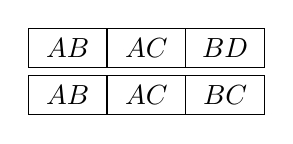
\begin{tikzpicture}[scale=1]
\draw (0,0.0) +(-.5,-.25) rectangle ++(.5,.25);
\draw (0,0.0) node{$A B$};x
\draw (1.0,0) +(-.5,-.25) rectangle ++(.5,.25);
\draw (1.0,0) node{$A C$};
\draw (2.0,0) +(-.5,-.25) rectangle ++(.5,.25);
\draw (2.0,0) node{$B C$};
\draw (0.0,.60) +(-.5,-.25) rectangle ++(.5,.25);
\draw (0.0,.60) node{$A B$};
\draw (1.0,.60) +(-.5,-.25) rectangle ++(.5,.25);
\draw (1.0,.60) node{$A C$};
\draw (2.0,.60) +(-.5,-.25) rectangle ++(.5,.25);
\draw (2.0,.60) node{$B D$};
\end{tikzpicture}
\end{figure}
For the first configuration, we can swap $A$ to be with its partner in either the first or second block:
\begin{figure}[H]
\centering
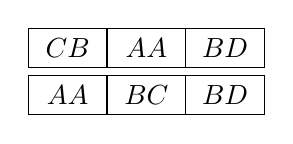
\begin{tikzpicture}[scale=1]
\draw (0,0.0) +(-.5,-.25) rectangle ++(.5,.25);
\draw (0,0.0) node{$A A$};
\draw (1.0,0) +(-.5,-.25) rectangle ++(.5,.25);
\draw (1.0,0) node{$B C$};
\draw (2.0,0) +(-.5,-.25) rectangle ++(.5,.25);
\draw (2.0,0) node{$B D$};
\draw (0.0,.60) +(-.5,-.25) rectangle ++(.5,.25);
\draw (0.0,.60) node{$C B$};
\draw (1.0,.60) +(-.5,-.25) rectangle ++(.5,.25);
\draw (1.0,.60) node{$A A$};
\draw (2.0,.60) +(-.5,-.25) rectangle ++(.5,.25);
\draw (2.0,.60) node{$B D$};
\end{tikzpicture}
\end{figure}
Other than changing which pair of seats are occupied, we have a happy couple $A$ and two pairs of unhappy patrons, $BC$ and $BD$.  These configurations require the exact same number of swaps to rectify.

If we instead swapped $B$, we'd get two configurations also:
\begin{figure}[H]
\centering
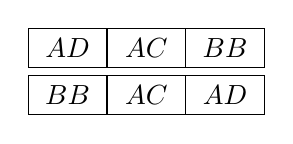
\begin{tikzpicture}[scale=1]
\draw (0,0.0) +(-.5,-.25) rectangle ++(.5,.25);
\draw (0,0.0) node{$B B$};
\draw (1.0,0) +(-.5,-.25) rectangle ++(.5,.25);
\draw (1.0,0) node{$A C$};
\draw (2.0,0) +(-.5,-.25) rectangle ++(.5,.25);
\draw (2.0,0) node{$A D$};
\draw (0.0,.60) +(-.5,-.25) rectangle ++(.5,.25);
\draw (0.0,.60) node{$A D$};
\draw (1.0,.60) +(-.5,-.25) rectangle ++(.5,.25);
\draw (1.0,.60) node{$A C$};
\draw (2.0,.60) +(-.5,-.25) rectangle ++(.5,.25);
\draw (2.0,.60) node{$B B$};
\end{tikzpicture}
\end{figure}

These cases are, exactly like the $A$ swapping cases, equivalent in terms of how many swaps would be required to finish pairing the rest of the plane.  The seconed possible initial case (where $A$ and $B$ are both seated next to family $C$, yields similarly equivalent situations after an exchange for $A$:
\begin{figure}[H]
\centering
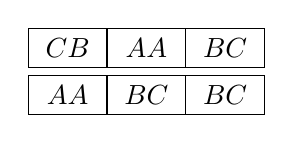
\begin{tikzpicture}[scale=1]
\draw (0,0.0) +(-.5,-.25) rectangle ++(.5,.25);
\draw (0,0.0) node{$A A$};
\draw (1.0,0) +(-.5,-.25) rectangle ++(.5,.25);
\draw (1.0,0) node{$B C$};
\draw (2.0,0) +(-.5,-.25) rectangle ++(.5,.25);
\draw (2.0,0) node{$B C$};
\draw (0.0,.60) +(-.5,-.25) rectangle ++(.5,.25);
\draw (0.0,.60) node{$C B$};
\draw (1.0,.60) +(-.5,-.25) rectangle ++(.5,.25);
\draw (1.0,.60) node{$A A$};
\draw (2.0,.60) +(-.5,-.25) rectangle ++(.5,.25);
\draw (2.0,.60) node{$B C$};
\end{tikzpicture}
\end{figure}

And $B$

\begin{figure}[H]
\centering
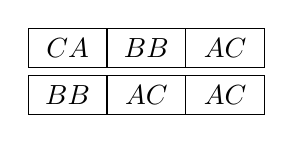
\begin{tikzpicture}[scale=1]
\draw (0,0.0) +(-.5,-.25) rectangle ++(.5,.25);
\draw (0,0.0) node{$B B$};
\draw (1.0,0) +(-.5,-.25) rectangle ++(.5,.25);
\draw (1.0,0) node{$A C$};
\draw (2.0,0) +(-.5,-.25) rectangle ++(.5,.25);
\draw (2.0,0) node{$A C$};
\draw (0.0,.60) +(-.5,-.25) rectangle ++(.5,.25);
\draw (0.0,.60) node{$C A$};
\draw (1.0,.60) +(-.5,-.25) rectangle ++(.5,.25);
\draw (1.0,.60) node{$B B$};
\draw (2.0,.60) +(-.5,-.25) rectangle ++(.5,.25);
\draw (2.0,.60) node{$A C$};
\end{tikzpicture}
\end{figure}

In all cases, exchanging either $A$ or $B$ first left us with conifgurations that were identical up to relabeling $A$ and $B$.  Further, swapping $A$ or $B$ out of the first pair into the seat beside its partner left us with identical configurations up to a reordering of seats.
\end{proof}

Since all sweep algorithms that make at least one couple happy with every exchange are equivalent, and there exists an optimal sweep algorithm that does exactly that, we have proven that our sweep alorithm finds the lowest number of required exchanges.

\subsection{Mixed families -- couples and singletons}

Let us now consider the case where we have a mixture of couples and singletons, where we want to seat all the couples together. We assume that singletons are always happy, irrespective of whom they sit next to.


\subsubsection{Phase One, determining structure:} 

We first observe that the worst case scenario for performing exchanges is when we have a situation like:

\begin{equation*}
eAABBCCDDe
\end{equation*}

This requires 4 swaps, or one swap per couple between the two unhappy members of the $e$ pair.  In terms of defining structure beforehand, this was an example of the following situation (where solid boxes will be occupied by a couple, and dotted by singletons):

\begin{figure}[H]
\centering
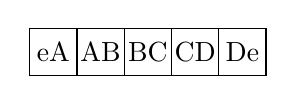
\begin{tikzpicture}[scale=1]
\draw (0.0,0) +(-.3,-.3) rectangle ++(.3,.3);
\draw (0.0,0) node{eA};
\draw (0.6,0) +(-.3,-.3) rectangle ++(.3,.3);
\draw (0.6,0) node{AB};
\draw (1.2,0) +(-.3,-.3) rectangle ++(.3,.3);
\draw (1.2,0) node{BC};
\draw (1.8,0) +(-.3,-.3) rectangle ++(.3,.3);
\draw (1.8,0) node{CD};
\draw (2.4,0) +(-.3,-.3) rectangle ++(.3,.3);
\draw (2.4,0) node{De};
\end{tikzpicture}
\end{figure}

With this assignment, we can clearly see that all passengers are seated in an incorrect seat to start. If instead the two $e$ passengers were singletons, then the following structural assignment would have allowed us to keep all passengers in their starting seats and require zero swaps.

\begin{figure}[H]
\centering
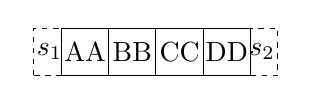
\begin{tikzpicture}[scale=1]
\draw[dash pattern= on 2pt off 2pt] (0,0) +(-.2,-.3) rectangle ++(.15,.3);
\draw (0.0,0) node{$s_1$};
\draw (0.45,0) +(-.3,-.3) rectangle ++(.3,.3);
\draw (0.45,0) node{AA};
\draw (1.05,0) +(-.3,-.3) rectangle ++(.3,.3);
\draw (1.05,0) node{BB};
\draw (1.65,0) +(-.3,-.3) rectangle ++(.3,.3);
\draw (1.65,0) node{CC};
\draw (2.25,0) +(-.3,-.3) rectangle ++(.3,.3);
\draw (2.25,0) node{DD};
\draw[dash pattern= on 2pt off 2pt] (2.7,0) +(-.15,-.3) rectangle ++(.2,.3);
\draw (2.7,0) node{$s_2$};
\end{tikzpicture}
\end{figure}

To properly assign a structure to a seating arangement for singletons and couples that minimizes swaps, we generalize the above bad example.  Sets of paired individuals already seating by their partners are known as blocks.  Our bad example had $AABBCCDD$ all starting in good places, and thus we had a block of $N = 4$ couples.  Our block was out of alignment with our first seating type assignment and would require $N$ swaps to satisfy all seating requirements.  On the other hand, the block was in perfect alignment with the second seating type assignment and required no swaps to be seated.

\begin{figure}[H]
\centering
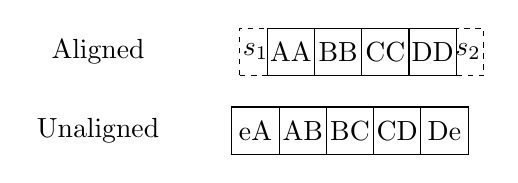
\begin{tikzpicture}[scale=1]
\draw (-2,0) node{Unaligned};
\draw (0.0,0) +(-.3,-.3) rectangle ++(.3,.3);
\draw (0.0,0) node{eA};
\draw (0.6,0) +(-.3,-.3) rectangle ++(.3,.3);
\draw (0.6,0) node{AB};
\draw (1.2,0) +(-.3,-.3) rectangle ++(.3,.3);
\draw (1.2,0) node{BC};
\draw (1.8,0) +(-.3,-.3) rectangle ++(.3,.3);
\draw (1.8,0) node{CD};
\draw (2.4,0) +(-.3,-.3) rectangle ++(.3,.3);
\draw (2.4,0) node{De};
\draw (-2,1) node{Aligned};
\draw[dash pattern= on 2pt off 2pt] (0,1) +(-.2,-.3) rectangle ++(.15,.3);
\draw (0.0,1) node{$s_1$};
\draw (0.45,1) +(-.3,-.3) rectangle ++(.3,.3);
\draw (0.45,1) node{AA};
\draw (1.05,1) +(-.3,-.3) rectangle ++(.3,.3);
\draw (1.05,1) node{BB};
\draw (1.65,1) +(-.3,-.3) rectangle ++(.3,.3);
\draw (1.65,1) node{CC};
\draw (2.25,1) +(-.3,-.3) rectangle ++(.3,.3);
\draw (2.25,1) node{DD};
\draw[dash pattern= on 2pt off 2pt] (2.7,1) +(-.15,-.3) rectangle ++(.2,.3);
\draw (2.7,1) node{$s_2$};
\end{tikzpicture}
\end{figure}


To fully represent a starting seating arrangement, we must note which passengers are not in blocks, contigious seats thus occupied will be called gaps.  While al blocks will be of even length (because they're comprised of couples), gaps can be of even or odd length.  I will refer to the parity of a gap as odd or even depending on whether the number of elements in it are odd or even.

\begin{lem} \label{lemma:ParityOnly}
For each starting block of size $N_i$, the optimal structural assignment will have a contiguous block of $N_i$ coupled seats. These can either be at the starting location or offset from that position by 1.
\end{lem}

\begin{proof}[Proof that contiguous blocks remainin in place.]
By contradiction.  Let's suppose that the first (left) $k$ couples are declared to be aligned improperly with seats asigned to couples, and the remaining $N-k$ to be aligned properly.  In order for this to occur, there had to be a singleton seat at the transition from aligned to unaligned.  

In order for this structural assignment to be optimal, there can't be a place to put this singleton that would require fewer swaps than the middle of this block.  However, placing it to the left of the $k$ unaligned couples would allow them to all be properly aligned, and reduce the number of swaps required by $k$.
\end{proof}

This in hand, we are going to ask how many existing blocks are going to have to be declared unaligned in order to globally minimize the number of swaps we perform. When a block is declared unaligned, we mean that instead of saying its first and second passengers (who are presupposed to be a couple due to this being a block) are in a single pair of couple designated seats, that instead they are siting in two different designated paired seats.  i.e.


We need another lemma before we can get an algorithm out of these observations.

\begin{lem} \label{lem:oddGapsNeedSingletons}
To satisfy all couples in an odd parity gap without disturbing its neighboring blocks, an odd number of singleton seats will be assigned to the gap.
\end{lem}

\begin{proof}
All seats not assigned to a singletons are assigned in pairs to couples.  All assigned couples take up an even number of seats leaving an odd number of seats to fill with singletons.
\end{proof}

\begin{cor}
All odd gaps require at least one singleton seat to be assigned to it.
\end{cor}

\begin{cor}
Any structural assignment with more odd parity gaps than singleton passengers will require that some blocks move.
\end{cor}

So which blocks move?  With $O$ representing a gap of odd parity, $E$ a gap of even parity, and $B$ being a block, the following situations exhaustively describe gap-block borders:

\begin{align*}
O B O \\
E B O \\
O B E \\
E B E \\
O B_1 E B_2 E B_3 \hdots B_k O \\
\end{align*}

In the first situation, if we declare the block unaligned and then perform the $N$ couple swaps to make it a block again, we wind up with $E B E$ and two fewer odd parity gaps.  

If we declare the block unaligned in the second or third cases, and preform $N$ couple swaps to make it a block again, we wind up with $O B E $ and $E B O$ respectively but keep the number of odd parity gaps constant.  The third case would become $O B O$, generating two aditional odd parity gaps.

The final case would become $E B_1 E B_2 E \hdots B_k E$.  This would reduce the number of odd parity gaps by 2 and cost $\sum_{i=1}^k |B_i|$ swaps.  Please note that only shifts between adjacent odd parity gaps decrease the number of odd parity gaps that we have, that all such shifts decrease our number of odd parity gaps by 2 and that they all cost a number of swaps equal to the number of couples in the blocks between them all.

\subsubsection{Dynamic Program for Gap Assignment}

A simple dynamic program can answer the question: which blocks do we declare unaligned in the optimal seating structure?  If the block between odd gap $i$ and $i+1$ has $N_i$ paired couples, then we label the number of required swaps to fix parity is $S(x,k)$ where $x$ is the index of the odd parity gap we're considering and $k$ is the number of odd parity gaps we've closed.

Diagramatically, we have:



Our recurrence relation is: 

\begin{equation*}
  S(x,k) = \min_x S(x-2, k-2) + N_{x}
\end{equation*}

Memoizing this table takes the number of odd gaps times the number of gaps we have to close.  Since each gap has to end with a block, the number of odd gaps is no more than $\frac13$ of our total number of seats.  Since we can't close more gaps than we have, this simple algorithm is, at worst, quadratic in number of passengers.  

\subsubsection{Phase Two: Performing the Swap Sweep}

With the block structure in hand from the first step of our algorithm, we can finally get down to the business of counting passenger swaps. 

\begin{algorithm}
  \caption{ \texttt{SwapScan} }
  \label{alg:swapScan}
  Number of singletons $numS$
  Number of odd parity gaps $numP$
  Sweep left to right over position $x_i$

  \uIf(\tcp*[h]{Leave them together}){ $x_i$ and $x_{i+1}$ are a pair}{    
    $i \leftarrow i + 2$\;
  }
  \uElseIf{ $x_i$ is part of a couple}{
    \uIf{ $x_{i+1}$ and $x_{i+2}$ aren't an already assigned pair}{
      Place $x_i$'s partner in $x_{i+1}$\;
      $i \leftarrow i + 2 $\;
    }    
    \Else( \tcp*[h]{Try to trade $x_i$ for a singleton} ) {     
      \uIf{ $x_i$'s partner is next to a singleton} {
        %%  This is wrong %%
        \uIf{ Left singleton $s_L$ is an even number of units from the end of the previous block,} {
          Exchange $x_i$ for $s_L$\;
          $numS \leftarrow numS-1$\;
        }
        \uElseIf{ Right singleton $s_R$ is an even number of units from the end of the next block} {
          Exchange $x_i$ for $s_R$\;
          $numS \leftarrow numS - 1$\;
        }      
        \Else{
          Exchange $x_i$ for the first singleton to its right.
          $numS \leftarrow numS - 1$\;
        } %even parity exchange possible 
      }
      \Else { %partner not next to a singleton
        Exchange $x_i$ for the first singleton to its right.\;
        $numS \leftarrow numS - 1$\;
      } %partner not next to a singleton
      \tcp*[h]{$numS$ unchanged: we already budgeted for this}
      $i \leftarrow i + 3$\;
    } % if next 2 are a couple
  }
  \Else( \tcp*[h]{$x_i$ is a singleton} ) {
    \uIf{ $x_{i+1}$ is half of a couple} {
      Place $x_{i+1}$'s partner in $x_i$\;
      $i \leftarrow i + 2$\;
    }
    \Else (\tcp*[h]{Enforce conservation of singletons} ) {      
      \uIf{$x_{i+1}$ is a singleton}{
            \uIf(\tcp*[h]{Leave these two singletons in their seats}){ $numS >= 2$}{              
              $numS \leftarrow numS - 2$\; 
              $i \leftarrow i + 2$\; 
            }
            \Else(\tcp*[h]{We have to swap them both out}){
              trade $x_i$ for the last unpaired couple in the plane\;
              trade $x_{i+1}$ for $x_i$'s partner\;
              $i \leftarrow i + 2$\;
            }
          }
          \Else{
            \uIf(\tcp*[h]{Leave one singleton in its seat}){$numS \geq 1$}{    
              $numS \leftarrow numS - 1 $\;
              $i \leftarrow i + 1 $\;
            }
            \Else{
              trade $x_i$ for the last unpaired couple in the plane\;
              $i \leftarrow i + 1$\;          
            }
          }
    }
  } % $x_i$ was a singleton

\end{algorithm}

\FloatBarrier
\section{Interesting Questions}

\begin{enumerate}
\item Problem with families of size 3? Families of mixed sizes?
\item Suppose we want to preserve certain seats qualities (aisle, window, etc)?
\item What if some type of seats people are averse to sit next to? For example, seats near crying babies or near toilets.
\item How do we minimize the maximum amount of movement for any one person?
\item How about two dimensional planes?
\item Aisle and window preference considerations?
\item Minimize total distance traveled?
\item Allow simultaneous swaps if no people in motion cross paths (other than those that are exchanging seats).  This is more fun if we have more than one aisle to walk down.
\end{enumerate}

\newpage
\section{References}

Algorithm reading group notes scribed by S Munson, September 2012.

\end{document}
